\section{Testfälle}
% TODO T Nummern anpassen


\subsection{Globale Testfälle}
Folgende Funktionssequenzen sind zu überprüfen:

\begin{itemize}
\item /T110/ Erstmaliges Starten des Programms
\begin{itemize}
\item Während das Programm sich im Ladebildschirm befindet, werden dem Spieler Comic-artige Sprechblasen mit lustigen und interessanten Texten angezeigt.
\item Der Nutzer startet das Programm und befindet sich im Sprachauswahlmenü $($Abb. \ref{fig:Sprachauswahlmenu}$)$. Mit den Sprachauswahl-Buttons $($S2$)$ wählt er die Sprache Deutsch aus.
\item Durch Drücken des Weiter-Buttons $($B1$)$ wechselt das Programm zum Namenswahlmenü $($Abb. \ref{fig:Namenswahlmenu}$)$. Hier wird der Spieler nach seinem Namen gefragt, den er in der Namenseingabe-Textbox eingibt.
\item Durch Drücken des  Weiter-Buttons $($B1$)$ wechselt das Programm zum Avatarauswahlmenü $($Abb. \ref{fig:Avatarauswahlmenu}$)$.
 Mit den Knöpfen A1 und A2 wählt er den gewünschten Avatar aus.
\item Durch Drücken des Weiter-Buttons $($B1$)$ erscheint der Begrüßungsbildschirm $($Abb. \ref{fig:Begrussungsbildschirm}$)$ mit Name und Avatar des Spielers.
\item Nach 3 Sekunden wechselt das Programm automatisch zum Hauptmenü $($Abb. \ref{fig:Hauptmenu}$)$.
\end{itemize}

\item /T120/ Starten des Programms, nachdem mindestens ein Profil bereits erstellt wurde
\begin{itemize}
\item Der Nutzer startet das Programm und befindet sich im Profilauswahlmenü $($Abb. \ref{fig:Profilauswahlmenu}$)$. Hier wählt er durch Drücken des Name-Button $($P1$)$, welcher mit seinem Namen beschriftet ist, sein Profil aus.
\item Es erscheint der Begrüßungsbildschirm $($Abb. \ref{fig:Begrussungsbildschirm}$)$ mit Name und Avatar des Spielers.
\item Nach 3 Sekunden wechselt das Programm automatisch zum Hauptmenü $($Abb. \ref{fig:Hauptmenu}$)$.
\end{itemize}

\item /T130/ Profildaten ändern
\begin{itemize}
\item Der Nutzer befindet sich im Profilauswahlmenü $($Abb. \ref{fig:Profilauswahlmenu}$)$.
\item Durch Drücken des Konfigurations-Buttons $($P2$)$ öffnet sich ein Dialog-Fenster, in dem der Nutzer die Option "`Profil editieren"' wählt. Das Programm wechselt zum Sprachauswahlmenü $($Abb. \ref{fig:Sprachauswahlmenu}$)$. 
\item Wie in /T110/ beschrieben gibt der Nutzer nacheinander Sprache, Namen und Avatar ein.
\item Nach Drücken des Bestätigungs-Buttons $($B3$)$ im Menü Avatarauswahlmenü $($Abb. \ref{fig:Avatarauswahlmenu}$)$ wechselt das Programm zurück in das Profilauswahlmenü $($Abb. \ref{fig:Profilauswahlmenu}$)$.
\end{itemize}

\item /T140/ Profil löschen
\begin{itemize}
\item Der Nutzer befindet sich im Profilauswahlmenü $($Abb. \ref{fig:Profilauswahlmenu}$)$.
\item Durch Drücken des Konfigurations-Buttons $($P2$)$ öffnet sich ein Dialog-Fenster, in dem der Nutzer die Option "`Profil löschen"' wählt.
\item In einem weiteren Dialog-Fenster bestätigt der Spieler seine Aktion.
\item Das Programm wechselt zurück in das Profilauswahlmenü $($Abb. \ref{fig:Profilauswahlmenu}$)$. Da das Profil jetzt gelöscht ist, erscheint es hier nicht mehr zur Auswahl.
\end{itemize}

\item /T150/ Beispiellevel zur Eingabe-Bestimmung
\begin{itemize}
\item Der Nutzer startet das Beispiellevel in Abbildung \ref{fig:Beispiellevel}.
\item Das Programm wechselt zum Editormodus $($Abb. \ref{fig:Editormodus}$)$ und es wird sofort ein Popup-Fenster angezeigt, in dem das Levelziel wie in Abbildung \ref{fig:Beispiellevel}b angezeigt wird.
\item Nach dem Schließen des Popups durch Berühren des Fensters sieht der Spieler den Editormodus $($Abb. \ref{fig:Editormodus}$)$ mit dem Term wie in Abbildung \ref{fig:Beispiellevel}a.
\item Durch Drücken des Hinweis-Buttons $($G2$)$ öffnet sich ein Popup-Fenster, in dem die Hilfestellung zum aktuellen Level wie in Abbildung \ref{fig:Beispiellevel}c angezeigt wird. Der Spieler schließt das Popup durch Berühren des Fensters.
\item Über die Drag\&Drop Geste wählt der Spieler einen weißen Edelstein von der Werkzeugleiste aus und zieht diesen an die Position G9 $($Abb. \ref{fig:Beispiellevel}a$)$. Bevor er den Zeiger loslässt, erscheint ein weißer Edelstein wie in Abbildung \ref{fig:Beispiellevel}c, aber jetzt transparent. Durch Loslassen des Zeigers wird der Edelstein an dieser Stelle im Term platziert, er ist jetzt also nicht mehr transparent.
\item Durch Drücken des neu hinzugefügten weißen Edelsteins öffnet sich ein Kontextmenü, in dem dem Spieler mehrere Farben zur Verfügung stehen. Er wählt die Farbe rot durch Drücken des entsprechenden Feldes aus, sodass der zuvor weiße Edelstein jetzt rot wird.
\item Der Spieler versucht das durch das Level bereits vorgegebene blaue Lamm durch die Drag\&Drop Geste auszuwählen und zu verschieben, das Programm unterdrückt dies aber.
\item Durch Drücken des Reduktions-Buttons $($G5$)$ wechselt das Programm mit dem gerade erstellen Term in den Reduktionsmodus $($Abb. \ref{fig:Reduktionsmodus}$)$.
\item Der Spieler drückt den Schritt-Vorwärts-Button $($R3$)$ und das Programm führt den ersten Reduktionsschritt $($Abb. \ref{fig:Beispiellevel_Reduktion}$)$ aus. Der Spieler kann eine Animation sehen, in der das rote Lamm den vor sich liegenden grünen Edelstein verzaubert. Dabei verschwindet der grüne Edelstein, es verwandeln sich beide rote Edelsteine in grüne Edelsteine, das rote Lamm verliert sowohl seinen Zauberstab als auch seine Farbe - erhält also die Farbe weiß - und verschwindet darauf auch vom Bildschirm. Der übriggebliebene Term rückt jetzt an die Stelle des roten Lamms.
\item Der Spieler drückt den Abspiel-Button $($R2$)$. Der automatische Abspielmodus startet und der Abspiel-Button erhält ein Pausesymbol. Das blaue Lamm verzaubert wie oben beschrieben den ersten vor sich liegenden, grünen Edelstein . Nach der Animation bleiben genau zwei nebeneinander stehende, grüne Edelsteine übrig. Es sind keine weiteren Reduktionsschritte möglich, der Abspiel-Button erhält wieder ein Abspielsymbol.
\item Die Reduktion ist fertig und der reduzierte Term gleicht dem Levelziel, das Level ist also bestanden. Es öffnet sich der Levelabschluss-Dialog $($Abb. \ref{fig:Reduktionsmodus_Levelabschluss}$)$.
\end{itemize}

\begin{figure}[H]
\centering

\begin{subfigure}{.3\textwidth}
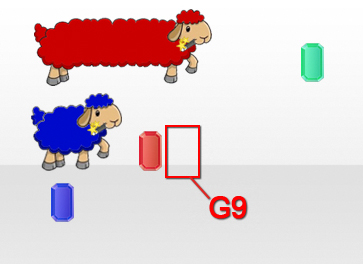
\includegraphics[width=\textwidth]{../gui/level_example/game_wog.jpg}
\caption{Anfangsanordnung}
\end{subfigure}
\begin{subfigure}{.3\textwidth}
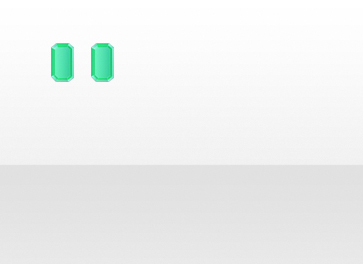
\includegraphics[width=\textwidth]{../gui/level_example/game_finish_wog.jpg}
\caption{Zielanordnung}
\end{subfigure}
\begin{subfigure}{.3\textwidth}
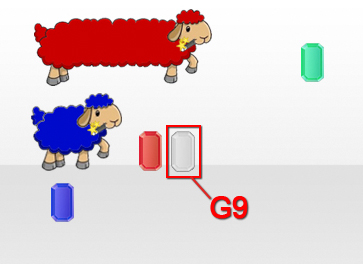
\includegraphics[width=\textwidth]{../gui/level_example/game_hint_wog.jpg}
\caption{Hinweis}

\end{subfigure}

\caption{Beispiellevel}
\label{fig:Beispiellevel}
\end{figure}

\begin{figure}[H]
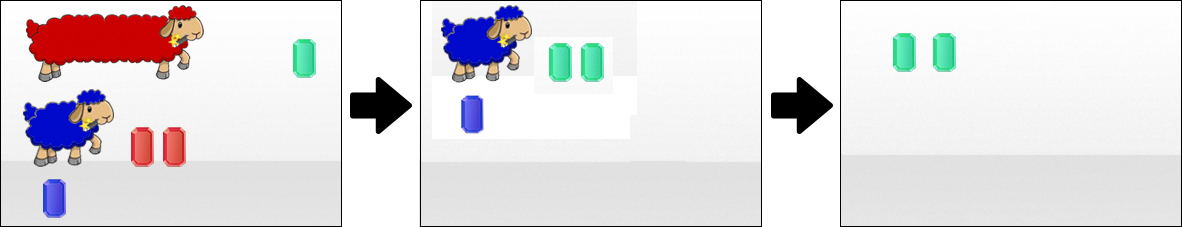
\includegraphics[width=\textwidth]{../gui/level_example/reduction123_wog.jpg}
\caption{Beispiellevel Reduktion}
\label{fig:Beispiellevel_Reduktion}
\end{figure}

\item /T160/ Level auswählen
\begin{itemize}
\item Der Nutzer befindet sich im Hauptmenü $($Abb. \ref{fig:Hauptmenu}$)$ und drückt den Level-Button $($H2$)$. Das Programm wechselt zum Levelauswahlmenü $($Abb. \ref{fig:Levelauswahlmenu}$)$.
\item Einige Level sind bereits abgeschlossen und durch einen Haken markiert, ein Level ist freigeschaltet und die restlichen Level nicht freigeschaltet und deshalb durch ein Schloss markiert. Level mit demselben Schwierigkeitsgrad sind hier farblich gleich gekennzeichnet.
\item Der Spieler wählt das erste Level durch Drücken des Levelstart-Buttons $($L1$)$ aus und das Programm wechselt in den Editormodus zur Bearbeitung dieses Levels.
\end{itemize}

\item /T170/ Das Einkaufsmenü benutzen
\begin{itemize}
\item Der Spieler besitzt durch Abschluss mehrerer Level eine Anzahl an Münzen. Bisher hat er noch keine Elemente im Shop gekauft.
\item Das Programm befindet sich im Hauptmenü $($Abb. \ref{fig:Hauptmenu}$)$. Durch Drücken des Einkaufs-Button $($H6$)$ wechselt es zum Einkaufsmenü $($Abb. \ref{fig:Einkaufsmenu}$)$.
\item Hier wählt der Spieler das Musik-Dropdownmenü $($E1$)$ aus. Es erscheinen mehrere zum Kauf verfügbare Objekte $($Abb. \ref{fig:Einkaufsmenu_Dropdown}$)$.
\item Der Spieler wählt den ersten Sound aus und wird darauf durch ein Dialog-Fenster zur Bestätigung des Kaufs gebeten.
\item Nach der Bestätigung wird der Sound freigeschaltet und automatisch aktiviert.
\item Durch Wiederholen dieser Schritte kauft er auch den zweiten verfügbaren Sound. Dieser wird automatisch aktiviert.
\item Der Spieler aktiviert nun wieder den ersten Sound, indem er auf das zweite Element drückt. Das aktivierte erste Element wird durch einen Haken gekennzeichnet, der Haken beim deaktivierten zweiten Element wird entfernt.
\end{itemize}

\item /T180/ Optionen auswählen
\begin{itemize}
\item Das Programm befindet sich im Hauptmenü $($Abb. \ref{fig:Hauptmenu}$)$. Durch Drücken der Stumm-Checkbox $($H5$)$ wird die Hintergrundmusik deaktiviert.
\item Durch Drücken des Optionen-Buttons $($H4$)$ wechselt das Programm in das Optionsmenü $($Abb. \ref{fig:Optionsmenu}$)$. Hier aktiviert der Spieler durch Drücken der Lehrermodus-Checkbox $($O1$)$ den Lehrermodus und durch Drücken der Farbenblindenmodus-Checkbox $($O2$)$ den Farbenblindenmodus.
\item Durch Verschieben des Geräusche-Sliders $($O4$)$ passt der Spieler die Geräuschelautstärke und durch Verschieben des Musik-Sliders $($O5$)$ die Musiklautstärke an.
\item Durch Drücken des Zurück-Buttons $($B2$)$ wechselt das Programm zurück in das Hauptmenü $($Abb. \ref{fig:Hauptmenu}$)$.
\end{itemize}

\item /T190/ Benutzerstatistik ansehen
\begin{itemize}
\item Das Programm befindet sich im Hauptmenü $($Abb. \ref{fig:Hauptmenu}$)$. Durch Drücken des Erfolge-Buttons $($H3$)$ wechselt das Programm in das Erfolgsmenü $($Abb. \ref{fig:Erfolgsmenu}$)$. Hier kann der Spieler seine abgeschlossenen Erfolge einsehen.
\item Durch Drücken des Zurück-Buttons $($B1$)$ wechselt das Programm zurück in das Hauptmenü $($Abb. \ref{fig:Hauptmenu}$)$.
\item Durch Drücken des Optionen-Buttons $($H4$)$ wechselt das Programm in das Optionsmenü $($Abb. \ref{fig:Optionsmenu}$)$.
\item Durch Drücken des Statistik-Buttons $($O3$)$ wechselt das Programm in das Statistikmenü $($Abb. \ref{fig:Statistikmenu}$)$. Hier kann der Spieler Statistiken zu seinem Spielverhalten einsehen.
\item Durch Drücken des Zurück-Buttons $($B2$)$ wechselt das Programm zurück in das Optionsmenü $($Abb. \ref{fig:Optionsmenu}$)$.
\item Durch Drücken des Zurück-Buttons $($B2$)$ wechselt das Programm zurück in das Hauptmenü $($Abb. \ref{fig:Hauptmenu}$)$.
\end{itemize}

\end{itemize}

\subsection{Datenkonsistenzen}
Folgende Datenkonsistenzen sind zu überprüfen:

\begin{itemize}
\item /T210/ Ein Profil ist eindeutig durch den Namen gekennzeichnet. Es kann nicht mehrere Profile mit demselben Namen geben.
\end{itemize}
